\chapter{Introdución}
\section{Contextualización}
Dende sempre o ser humano tivo inquietude por coñecer e entender como funciona o medio que o rodea, tarefa para a que resulta imprescindible a observación do mesmo. A observación defínese como a captación activa e rexistro de información dende unha fonte primaria, a través dos sentidos ou da utilización de instrumentos.

Dado o crecente interese polo estado do medio ambiente e os avances tecnolóxicos que se produciron nas últimas décadas, na actualidade xérase a cada instante unha inxente cantidade de datos que rexistra medicións dunha ampla variedade de fenómenos, empregando para elo os máis diversos métodos, dende modernos sensores montados en satélites ata o rexistro manual das medicións realizadas por un sinxelo termómetro de mercurio.

As maiores dificultades para converter este gran volume de datos en información útil son debidas a heteroxeneidade dos mesmos, tanto pola súa natureza física como polos medios empregados para capturalos e rexistralos.

Para atallar este problema xurdiu dende o Open Geospatial Consortium\footnote{O OGC é un consorcio formado por máis de cincocentas empresas privadas, universidades e axencias gobernamentais co obxectivo de desenvolver e publicar estándares no eido da información xeoespacial (\url{http://www.opengeospatial.org/} e \url{https://www.youtube.com/watch?v=bfkCdir-yO8}).}(OGC) a iniciativa Sensor Web Enablement (SWE), que ten como obxectivo principal a estandarización de modelos, formatos e interfaces que teñan que ver coa xestión de información de observación medioambiental. De importancia para o presente traballo de fin de grado son os estándares Observations and Measurements (O\&M) e Sensor Observation Service (SOS).

O estándar O\&M define un modelo de datos e a súa codificación XML para a representación de observacións medioambientais. Cada observación modelada en O\&M proporciona un valor observado para unha propiedade concreta (Observed Property) dunha entidade observada (Feature Of Interest - FOI). Por exemplo, un valor real para a temperatura (Observed Property) dunha estación meteorolóxica (FOI). Outros metadatos asociados á observación son, por exemplo, o instante de tempo no que a observación se aplica á FOI (Phenomenon Time) e o proceso utilizado para xerar a observación. O proceso utilizado normalmente é a combinación de algún dispositivo físico (Sensor) con algún algoritmo de procesamento; por exemplo, para calcular a temperatura diaria na estación combinase un sensor de temperatura que ofrece medidas cada dez minutos con un algoritmo de agregación de datos.

O estándar SOS define a interface do servizo web que permite consultar observacións, metadatos dos sensores e a representación das entidades observadas. Amais define os medios para rexistrar novos sensores ou eliminar os existentes, así como para inserir novas observacións para os sensores rexistrados. Este estándar apoiase en outros, tamén desenvolvidos polo OGC, que definen os modelos para a representación dos datos a comunicar, así pois as xeometrías das entidades observadas represéntase a través do Geography Markup Language (GML), os metadatos dos sensores a través do SensorML e as observacións a través do xa citado Observations and Measurements (O\&M).

As observacións de fenómenos medioambientais son, polo tanto, un tipo de información xeográfica; de feito para poder interpretar os datos de observacións de forma correcta, durante os procesos de apoio á toma de decisións, é fundamental dispoñer de metadatos que proporcionen o seu contexto temporal e espacial. Como se describiu anteriormente, o contexto temporal ven proporcionado polo Phenomenom Time, mentres que o contexto espacial ven dado polas propiedades de tipo xeográfico dispoñibles na FOI. Pódese abordar, polo tanto, a análise e explotación destes datos empregando como ferramenta un Sistema de Información Xeográfica (SIX) de propósito xeral.

Un SIX é un sistema deseñado para capturar, almacenar, manipular, analizar e presentar calquera tipo de información xeograficamente referenciada. Dentro do software SIX distínguense varios grandes grupos segundo o seu propósito, como poden ser sistemas de xestión de bases de datos espaciais, servidores cartográficos, visores web, móbiles ou de escritorio. Dentro deste último grupo, os SIX de escritorio, inclúense un amplo número de programas que permiten visualizar, editar e analizar datos xeográficos e que se empregan en moitos eidos e con moi diversos fins, por exemplo para investigacións científicas, meteoroloxía, cartografía, hidroloxía, xestión de recursos, marketing, loxística, avaliación do impacto ambiental, etc.

Os SIX traballan principalmente con dous formatos de información, segundo os obxectos do mundo real que se vaian representar sexan de natureza continua ou discreta. Así pois, para representar unha variable de natureza continua, como por exemplo un mapa da elevación do terreo, empregase o formato raster, que divide o espazo en celas regulares asociando un valor a cada unha delas. Pola contra, para representar obxectos de natureza discreta, como pode ser un río, emprégase xeralmente o formato vectorial, no que se representa a xeometría en base a puntos, liñas ou polígonos, e se lle asocian a esta xeometría os atributos e valores que sexan necesarios. Cabe destacar que estes dous formatos poden converterse entre si se en función da análise a realizar, por exemplo, en base ás observacións de temperaturas en determinados puntos pódese xerar por interpolación un raster que represente o mapa térmico da zona (rasterización), ou pola contra, a partir dun mapa de elevación pódense trazar as curvas de nivel que o representan (vectorización).

En canto ás ferramentas de análise proporcionadas polos paquetes SIX, existe unha moi ampla gama de técnicas que se desenvolveron principalmente no último medio século, e é un campo que cambia rapidamente na actualidade, incluíndose cada vez máis e máis ferramentas, ben proporcionadas polo propio provedor orixinal do software ou en moitos casos desenvolvidas por terceiros a través das posibilidades de ampliación que os propios programas SIX poñen a disposición dos desenvolvedores.

Na maioría dos SIX o modelado dos fenómenos xeográficos realizase de forma estática, sen embargo na actualidade requírense modelos que engadan o tempo como variable, de xeito que permitan observar o comportamento dinámico dos eventos xeográficos, como por exemplo no caso das observacións de fenómenos medioambientais. Os SIX que incorporan a representación do tempo, amais das dimensións espaciais, denomínanse SIX temporais e permiten facer unha representación da información en 4D, o que abre un amplo abano de posibilidades. A incorporación da compoñente temporal é un dos aspectos o que máis esforzos se están a adicar actualmente, no que a evolución dos SIX se refire.

\section{Motivación e Obxectivos}

Na actualidade, a area de análise e explotación da información obtida a través das observacións medioambientais está moi fragmentada. Cada organismo ou axencia desenvolve as súas propias solucións para a captación, o almacenamento e a análise das cada vez máis amplas redes de sensores despregadas por todo o planeta. Este feito supón unha gran limitación en canto ó aproveitamento de toda esta información, o restrinxir o acceso á mesma as organizacións que dispoñen dos recursos necesarios para desenvolver e implantar os sistemas necesarios.

O estándar SOS pretende permitir a interoperabilidade entre os sistemas encargados de captar e almacenar esta información e os sistemas empregados para a análise da mesma, non obstante o grao de implantación deste estándar é aínda reducido. Como motivo, ou consecuencia, deste baixo grao de implantación existen na actualidade moi poucos sistemas de información xeográfica que inclúan o servizo SOS como unha fonte de datos soportada, a diferenza de outros estándares desenvolvidos polo OGC que son soportados pola ampla maioría dos sistemas, como o Web Map Service (WMS) ou o Web Feature Service (WFS).

As escasas solucións dispoñibles para operar con datos de observación servidos pola interface SOS en sistemas de información xeográfica pasan polo uso de extensións de terceiros para software comercial, como por exemplo ArcGIS\footnote{\url{http://www.esri.es/es/productos/arcgis/}}, que supón un elevado custe de licencia.

Este proxecto ven motivado, por tanto, pola inexistencia dun sistema de información xeográfica libre e de propósito xeral que permita a incorporación e análise de datos de observacións dispoñibles a través da interface SOS.

O obxectivo deste traballo é o desenvolvemento dunha extensión para a ferramenta SIX libre QGIS\footnote{\url{http://www.qgis.org/}} que permita a conexión a fontes de datos SOS e a exploración dos seus contidos no contorno de mapas proporcionado pola ferramenta.

\section{Entorno tecnolóxico}
\subsection{QGIS}
QGIS é un Sistema de Información Xeográfica de escritorio multiplataforma, libre e de código aberto. É un proxecto oficial da organización non gubernamental Open Source Geospatial Foundation\footnote{\url{http://www.osgeo.org/}} (OSGeo) nacido no ano 2002 co obxectivo principal de proporcionar unha ferramenta que permitise visualizar, editar e analizar datos xeográficos en calquera ordenador persoal.

Amais de proporcionar de por si soporte para un amplo número de formatos de datos e funcionalidades para operar cos mesmos, QGIS proporciona unha API completa para implementación de \emph{plugins} que amplíen a funcionalidade da ferramenta e os formatos de información xeográficos soportados. Os \emph{plugins} poden programarse en C++ ou en Python, e no caso de cumprir a normativa e ser aprobados polos responsables poden incluírse no repositorio oficial da aplicación, de xeito que se podan instalar directamente dende o propio QGIS.

QGIS é na actualidade o SIX libre de referencia, está apoiado por un gran número de organizacións que patrocinan o proxecto, e que son, xunto coas doazóns puntuais de particulares e organizacións o método de financiamento do proxecto. Arredor do QGIS desenvolveuse unha ampla e activa comunidade tanto de usuarios como de desenvolvedores, do propio QGIS ou de \emph{plugins}.

\subsection{Sensor Observation Service}
O estándar Sensor Observation Service\footnote{\url{http://www.opengeospatial.org/standards/sos}} define a interface do servizo web para descubrir e recuperar datos en tempo real ou arquivados producidos por calquera clase de sensor, tanto móbiles como estacionarios, in-situ ou remotos. Os datos dos sensores poden ser tanto observacións realizadas como descricións dos sensores ou metadatos dos mesmos relativos a calibracións, mantementos, etc. As observacións devólvense codificadas segundo o estándar Observations and Measurements, e a información sobre sensores a través de SensorML. O SOS define, na súa versión 1.0, tres grupos de operacións:
\begin{description}
\item[Core:] Estas operacións deben ser implementadas obrigatoriamente por todos os servizos SOS.
\begin{itemize}
\item \textit{GetCapabilities:} Esta operación é a que proporciona a descrición das capacidades do SOS, ademais de información xeral sobre o propio servizo. Entre outros datos indica as versións de SOS soportadas, os datos identificativos do servizo e do provedor do mesmo, as operacións que implementa (cos parámetros soportados por cada unha delas), os filtros soportados e a lista de ofertas provistas polo servizo, con información detallada de cada unha delas.
\item \textit{DescribeSensor:} Proporciona información relativa ó sensor requirido, segundo o estándar Sensor Model Language (SensorML). Entre outra información indícase a posición, nome e descrición do sensor ou sistema, o instante temporal da instalación e se proporciona medidas válidas, os fenómenos que pode medir e as unidades nas que os mide, e outra información relacionada, como un breve historial de reparacións e
calibracións, etc
\item \textit{GetObservations:} É a operación encargada de proporcionar os datos medidos polos sensores dunha determinada oferta e que cumpran os filtros definidos na consulta. Os valores destas observacións realizadas polos sensores devólvense segundo o estándar Observations and Measurements (O\&M). Este estándar define un formato de XML no que cada observación se describe polo fenómeno que mide, o sensor que o mide, o instante temporal da medida, a posición e nome do lugar no que se toma a medida e a unidade na que se mide o valor correspondente.
\end{itemize}
\item[Transactional:] Son as operacións que permiten rexistrar información no servizo. A súa implementación é opcional.
\begin{itemize}
\item \textit{RegisterSensor:} Permite rexistrar un novo sensor no servizo, mandando a súa descrición no formato SensorML.
\item \textit{InsertObservation:} Permite ó cliente inserir novas observacións no sistema de sensores previamente rexistrados.
\end{itemize}
\item[Extended:] Son operacións adicionais opcionais, para requirir información ó servizo.
\end{description}

A figura \ref{fig:uml-sos} representa a interacción entre un consumidor e os servizos SOS que interroga.

\begin{figure}[hbtp]
  \centering
  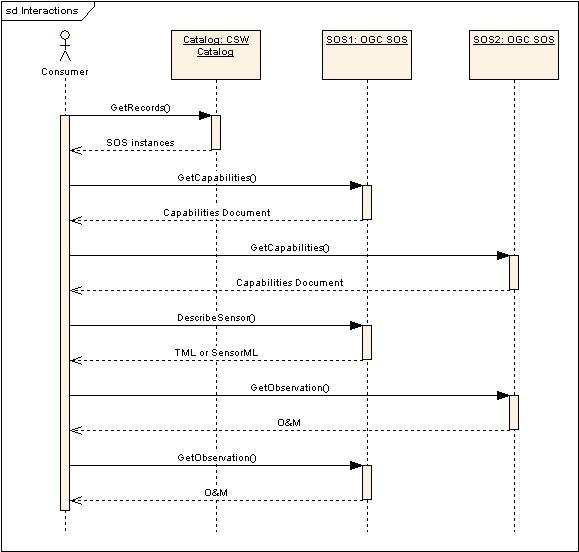
\includegraphics[width=.85\textwidth]{images/SOS_consumer_seq.png}
  \caption{Diagrama de secuencia dun consumidor SOS}
  \label{fig:uml-sos}
  \captionsetup{font={scriptsize,it}}
  \caption*{Fonte: \url{http://www.ogcnetwork.net/SOS_Intro}}
\end{figure}

\subsection{Observations and Measurements}
O estándar Observations and Measurements\footnote{\url{http://www.opengeospatial.org/standards/om}} define o modelo de datos e a súa codificación XML para a representación de observacións medioambientais. Define polo tanto modelos de documentos para o intercambio de información que describe o proceso de observación e os seus resultados entre diferentes comunidades técnicas e científicas.

Constitúe unha dependencia esencial para o estándar SOS.

O modelo de datos proposto é o que se mostra na figura \ref{fig:uml-om}.
\begin{figure}[hbtp]
  \centering
  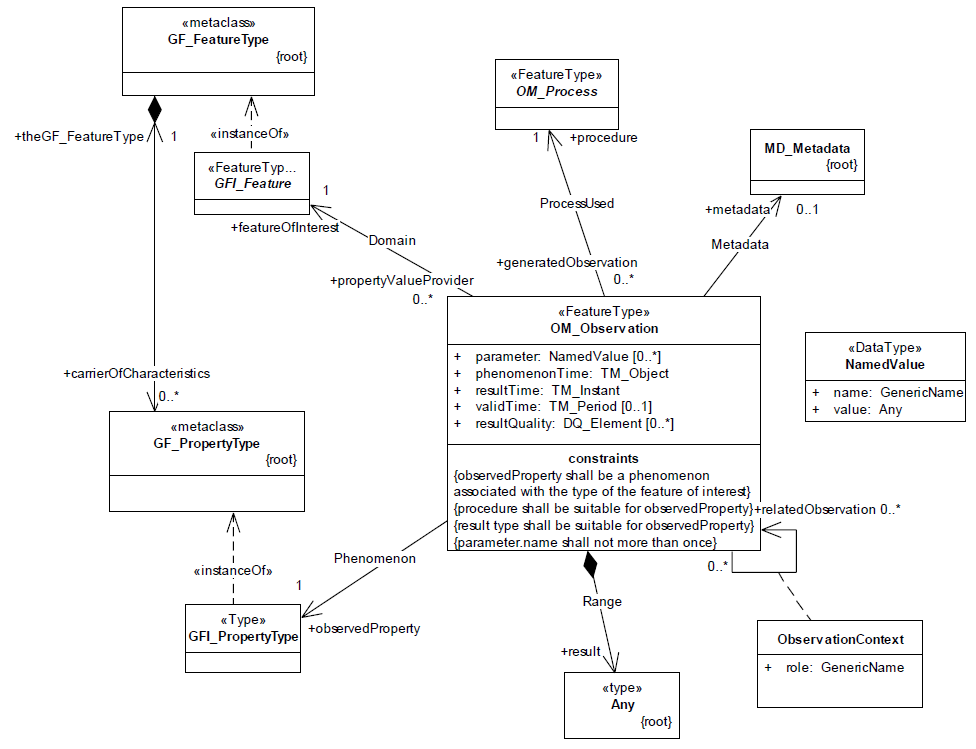
\includegraphics[width=.85\textwidth]{images/uml-observations.png}
  \caption{Diagrama UML dunha Observation}
  \label{fig:uml-om}
  \captionsetup{font={scriptsize,it}}
  \caption*{Fonte: \url{http://www.opengis.net/doc/IS/om-eo-metadata}}
\end{figure}

Segundo o modelo, unha observación é un evento que estima unha propiedade observada (Property) dalgunha entidade de interese (Feature Of Interest), utilizando un procedemento especificado (Process) e xera un resultado (Result).

\begin{description}
\item[Feature Of Interest:] Representa a entidade de interese ou área observada. Por exemplo, unha estación meteorolóxica. 
\item[Property:] Representa o fenómeno físico observado. Existen varios tipos, sendo o máis habitual o \emph{Measurement}, que é a combinación de un valor numérico real con unha unidade de medida. Por exemplo, a temperatura.
\item[Process:] Describe o proceso empregado para xerar o resultado. Pode ser un sensor, un conxunto de sensores, un algoritmo, etc. Por exemplo, un termómetro; ou ben, un algoritmo de agregación que calcule temperaturas medias, mínimas e máximas para un día.
\item[Result:] É o valor obtido para a propiedade observada na entidade de interese, obtido aplicando o procedemento indicado. Por exemplo, o rexistro de temperatura media para unha estación meteorolóxica nun día concreto.
\end{description}

\section{Estrutura da memoria}

Este documento estrutúrase en 6 capítulos, un apéndice e a bibliografía empregada.\\

Neste capítulo de introdución descríbese a motivación e obxectivos do proxecto e contextualizase o mesmo describindo brevemente os conceptos empregados e a situación actual da técnica nas areas de coñecemento relacionadas.\\

No capítulo 2 abórdanse os aspectos relativos á xestión do proxecto: a definición do alcance, a metodoloxía, planificación temporal e xestión de riscos e da configuración.\\

No capítulo 3 detállase a análise do software, describindo os casos de uso identificados e os requisitos extraídos dos mesmos.\\

No capítulo 4 descríbese o deseño do software, tanto a arquitectura do mesmo como o comportamento de cada unha das compoñentes.\\

No capítulo 5 documéntase en orde cronolóxico o proceso de deseño e implementación, así como as probas realizadas para cumprir os requisitos establecidos.\\

No capítulo 6 expóñense as conclusións extraídas de todo o proxecto e detállanse varias propostas de traballo futuro.\\
%\item[Apéndice A:] \textit{Manual técnico.}

O apéndice A é unha guía para a instalación e manexo básico do \emph{plugin} desenvolvido.\\
